%======================================================================
%  CRESCO8: the cluster and the observed configuration of its HBM nodes
%======================================================================

\section{CRESCO8}
\label{sec:cresco8}

CRESCO8 is an ENEA compute system at the Portici research centre, in
service since 2025~\cite{cresco8doc,eneapress}.  It has three classes of
compute node (\tabref{tab:cresco8-node-classes}).  This thesis uses the
CPU--HBM class; the general CPU class matters only as a possible
system-level baseline.

\begin{table}[htbp]
\centering
\footnotesize
\tabsetup
\begin{tabularx}{\textwidth}{P{1.55cm}P{1.05cm}P{1.45cm}P{2.65cm}Y}
\headrow
\headcell{Class} & \headcell{Nodes} & \headcell{CPU cores}\newline\headcell{per node}
 & \headcell{Memory}\newline\headcell{per node} & \headcell{Processor or accelerator} \\[3pt]
\tabheadrule
\tabstripeRow
CPU
 & 760 & 128 & 512\,GB DDR5
 & 2$\times$ Xeon Platinum 8592+ \\[3pt]

\tabrowsep
\tabplainRow
CPU--HBM
 & 16 & 112 & 1{,}024\,GB DDR5\newline + 128\,GB HBM
 & 2$\times$ Xeon CPU Max 9480 \\[3pt]

\tabrowsep
\tabstripeRow
GPU
 & 17 & 128 & 512\,GB DDR5\newline + accelerator HBM
 & 2$\times$ Xeon Platinum 8592+ and
   4$\times$ Intel Data Center GPU Max 1550 \\[3pt]
\tabbottomrule
\end{tabularx}
\caption{CRESCO8 node classes.  The CPU and GPU rows follow the ENEAGRID
documentation~\cite{cresco8doc}.  The CPU--HBM count is the scheduler's:
on 11 October 2026 Slurm listed 16 HBM nodes, whereas the documentation
lists 15.}
\label{tab:cresco8-node-classes}
\end{table}

The general CPU nodes are not a clean control for the HBM nodes.  The
Platinum 8592+ is an Emerald Rapids processor, one generation newer than
the Max 9480, with 64 cores, DDR5-5600 memory and a 320\,MB last-level
cache, nearly three times the Max 9480's 112.5\,MB~\cite{intel8592}.  A
comparison between the two node classes changes the core count, the
memory speed and the cache size together with the absence of HBM.  The
cache difference is the most serious confound for inference: the weights
of a model of a few hundred million parameters at 4-bit precision fit
almost entirely in the 8592+'s cache, which is the cache-residency effect
that Zhang et al.\ exploit~\cite{zhang2026cacheresident}.  Such a
comparison is therefore reported, if at all, as a system-level baseline
and never as an HBM effect.

\subsection{Interconnect}

Each HBM node has an NVIDIA ConnectX-7 adapter with one InfiniBand port
active at 200\,Gb/s, the NDR200 rate.  That is 25\,GB/s in each
direction: about a fortieth of one socket's nominal HBM bandwidth and a
twelfth of its DDR5 interface peak (\tabref{tab:xeon-max-peaks}).
Distributing a model
across nodes would make the network, not the memory tier, the dominant
cost, which is one reason the experiments stay within one node.

\subsection{Scheduler and allocation policy}
\label{sec:cresco8-scheduler}

Compute nodes are reached only through Slurm; the front-end nodes are
for editing, compilation and submission, not for measurement.  The HBM
nodes are split between two partitions with disjoint node lists.
\texttt{cresco8\_hbm} contains \texttt{cresco8-hbm01} to \texttt{hbm14},
with a 24-hour limit and a quality-of-service limit of five nodes per
user.  \texttt{cresco8\_hbm\_dbg} contains \texttt{hbm15} and
\texttt{hbm16}, with a one-hour limit.

The scheduler (Slurm 25.11.8) allocates individual cores
(\texttt{select/cons\_tres} with \texttt{CR\_CORE}) and does not allow jobs
of different users to be excluded from a node unless a job asks for it.
Without \texttt{-{}-exclusive}, another user's job can therefore run on the
other cores of the same node and compete for the same memory bandwidth
and, in Cache mode, the same HBM cache.  Every measurement in this thesis
uses an exclusive allocation.  Jobs run inside cgroup-v2 containers with
core and memory confinement: a job may use only the memory it requests,
and 10\,GB per node are reserved for the system.  The memory set of the
cgroup, by contrast, is not restricted (\secref{sec:hbm-clustering}).

\subsection{Storage and model staging}
\label{sec:cresco8-storage}

ENEAGRID provides AFS for home directories and the Lustre file system
\texttt{/lpor1}, 6.9\,PB in size and 90\% occupied at the time of the
check, for parallel I/O~\cite{cresco8doc}.  Each HBM node also has a
960\,GB Micron 7450 NVMe drive.  It holds the operating system, and its
root file system, including \texttt{/tmp}, had 104\,GB free; Slurm does
not manage it as a resource.  \texttt{/dev/shm} is a memory-backed file
system of up to 504\,GB.

Where the model file lives affects the measurement.  Runtimes such as
\lcpp{} map the model file into memory by default, so the weights become
page-cache pages of a Lustre file.  Those pages can be evicted and fetched
again over the network during a run, and their placement is decided when
they are first read rather than by the experiment's binding.  Models are
therefore staged to node-local storage before a run, and the weights are
loaded into anonymous memory (for \lcpp{} with \texttt{-{}-no-mmap}) so
that the binding applies to them.  The staging method is recorded with
each result.

\subsection{Software environment}
\label{sec:cresco8-software}

The HBM nodes run Red Hat Enterprise Linux~9.4 with kernel
5.14.0-427.13.1.  The kernel is booted with \texttt{mitigations=off} and
\texttt{intel\_pstate=disable}, and a site-specific \texttt{tuned}
profile is active.  The system compiler is GCC~11.4.1.  Environment
modules provide GCC~12, 14 and 15.1 and the Intel oneAPI 2025, 2025.3
and 2026.1 toolchains; oneAPI and an Intel-built Open MPI are loaded at
login by default.  \texttt{hwloc}~2.4.1 and \texttt{numactl} are
installed.  The versions of the inference runtimes and their libraries
are fixed per experiment, as described in the methodology.

\subsection{Observed configuration of the HBM nodes}
\label{sec:cresco8-observed}

The configuration of the regular HBM partitions was captured on
\texttt{cresco8-hbm15} by an exclusive job on 11 October 2026, with the
probes listed in \appref{app:reproducibility}.  The same probes are part
of the platform record that the benchmark suite stores with every
campaign~\cite{hwbench2026}, so each measurement in the following
chapters carries its own copy of this table.  An earlier allocation on
the same node, on 29 September 2026, had already shown two NUMA nodes and
no separate HBM node.  \tabref{tab:cresco8-manifest} lists what was
observed and why each item matters for the experiments.

\begin{table}[htbp]
\centering
\small
\tabsetup
\begin{tabularx}{\textwidth}{P{2.7cm}P{5.0cm}Y}
\headrow
\headcell{Item} & \headcell{Observed} & \headcell{Consequence} \\[3pt]
\tabheadrule
\tabstripeRow
Memory mode
  & Cache: two NUMA nodes of 503\,GB, each behind a 64\,GiB direct-mapped,
    write-back memory-side cache with 64\,B lines
  & HBM use is decided by footprint and physical placement, not by
    binding. \\[3pt]

\tabrowsep
\tabplainRow
Clustering
  & Quadrant: one NUMA node per socket
  & Binding is per socket. \\[3pt]

\tabrowsep
\tabstripeRow
DDR5 population
  & Eight 64\,GB DIMMs per socket, one per channel
  & All eight channels available. \\[3pt]

\tabrowsep
\tabplainRow
Threads
  & SMT inactive; 112 logical CPUs, one per core
  & Thread count equals core count. \\[3pt]

\tabrowsep
\tabstripeRow
Frequency control
  & \texttt{acpi-cpufreq} driver, \texttt{schedutil} governor
  & Frequency is not fixed; it is sampled during runs. \\[3pt]

\tabrowsep
\tabplainRow
NUMA balancing
  & Disabled; memory-tier demotion disabled
  & The kernel does not migrate pages behind the experiment. \\[3pt]

\tabrowsep
\tabstripeRow
Zone reclaim
  & \texttt{zone\_reclaim\_mode} = 1
  & A full local node reclaims page cache before allocating remotely. \\[3pt]

\tabrowsep
\tabplainRow
Huge pages
  & Transparent huge pages \texttt{always}; defragmentation on
    \texttt{madvise}
  & Large allocations get 2\,MB pages when free memory allows. \\[3pt]

\tabrowsep
\tabstripeRow
Counters and energy
  & \texttt{perf\_event\_paranoid} = 2; no \texttt{perf}; MSR and RAPL
    readable by root only
  & No uncore traffic or RAPL energy for users
    (\secref{sec:sd650-node}). \\[3pt]

\tabrowsep
\tabplainRow
Job cgroup
  & \texttt{cpuset.mems.effective} = \texttt{0-1}
  & Memory binding is not restricted by Slurm. \\[3pt]
\tabbottomrule
\end{tabularx}
\caption{Configuration of a CRESCO8 HBM node as observed by an exclusive
job on \texttt{cresco8-hbm15}, 11 October 2026.}
\label{tab:cresco8-manifest}
\end{table}

\figref{fig:cresco8-lstopo} is the topology reported by \texttt{lstopo}
on the same node.  It confirms the Cache-mode picture: each package has
one NUMA node of about 503\,GB, and the 64\,GB HBM appears only as a
\texttt{MemCache} object in front of it, never as allocatable memory.

\paragraph{The Flat-mode node.}  In addition to the regular partitions,
one HBM node has been configured in Flat mode with Quadrant clustering
for this work and is reached outside the regular partitions.  Its NUMA
topology has the four nodes
expected from \tabref{tab:hbm-six-configurations}: two CPU-bearing DDR5
nodes of about 503\,GiB and two memory-only HBM nodes of 64\,GiB, one per
socket.  The firmware's distance from a socket's cores to its local HBM
node is 13, and to the other socket's HBM node 23~\cite{hwbench2026}.
Flat-mode placement experiments run on this node; the node identifiers
are read from the running system before each run rather than assumed.

\begin{figure}[htbp]
\centering
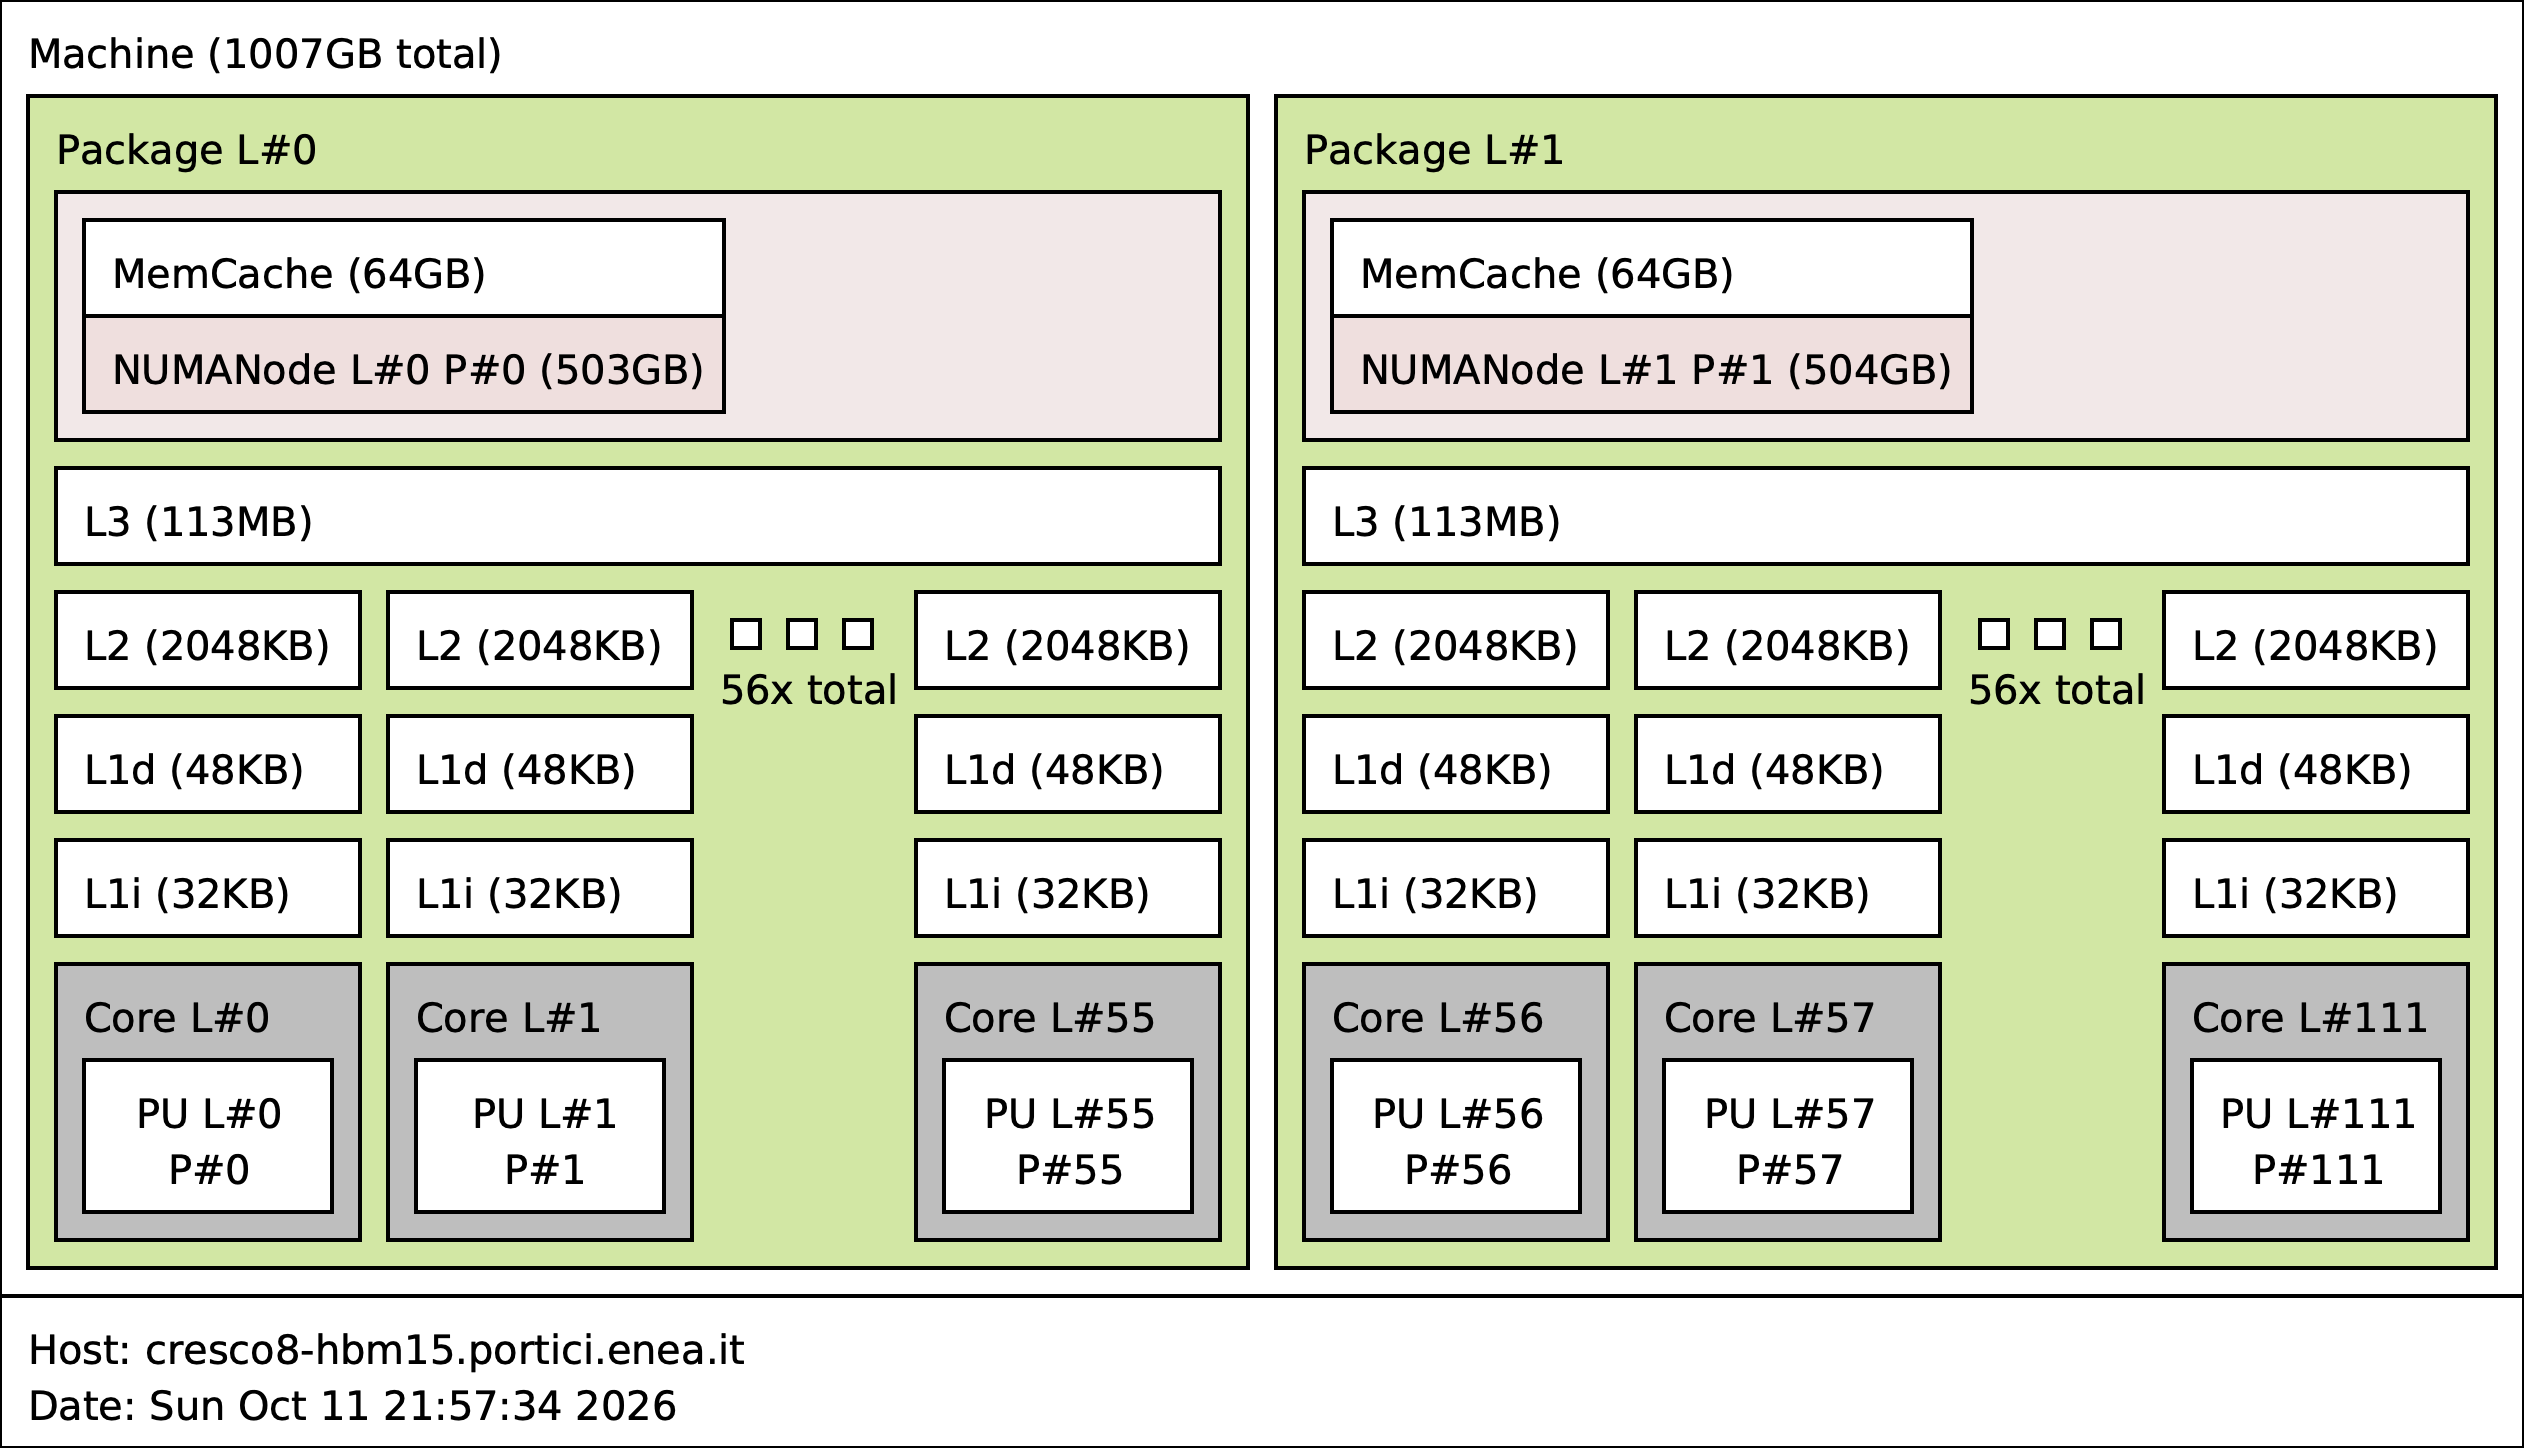
\includegraphics[width=0.9\textwidth]{cresco8-hbm-node-lstopo.png}
\caption{Topology of \texttt{cresco8-hbm15} as reported by
\texttt{lstopo} (hwloc~2.4.1) on 11 October 2026.  Two packages of 56
cores, each with a 113\,MB L3 and one DDR5 NUMA node behind a 64\,GB
memory-side cache (\texttt{MemCache}): the signature of Cache mode with
Quadrant clustering.}
\label{fig:cresco8-lstopo}
\end{figure}

\subsection{Why this platform}
\label{sec:why-cresco8}

Systems that combine HBM and DDR on a general-purpose CPU are rare, and
the largest, Aurora, is the source of most published measurements on the
Xeon Max~\cite{ibeid2025aurora,goto2026aurorahpl} but is not available to
this work.  CRESCO8's 16 HBM nodes provide access to the processor and
both of its local memories, and the experiments need only one socket at a
time.  The platform also sets a constraint.  Memory and clustering modes
are fixed at boot and the nodes are shared with other users, so the
configuration is not a per-job variable.  Two configurations are
available: Cache with Quadrant clustering on the regular partitions, and
Flat with Quadrant clustering on one dedicated node.  SNC4 and HBM-only
would each be a separate block of experiments arranged with the
administrators.
